\chapter{寄生虫病}

\chapterabstract{本章主要介绍阿米巴病和血吸虫病。要求掌握阿米巴病和血吸虫病的基本病变;熟悉血吸虫病的临床病理联系;了解阿米巴病、血吸虫病的病因及发病机制。}

寄生虫病(Parasitosis)是由寄生虫寄生于人体后引起的一类疾病的总称。寄生虫病的流行不仅与生物因素有关,而且与自然因素和社会因素关系密切,具有地理分布的区域性、明显的季节性和自然疫源性等特点。寄生虫病的流行需要三个条件:传染源(被寄生虫感染的人或动物)、传播途径(适宜寄生虫生活的环境条件、感染途径和感染方式)以及易感人群(对寄生虫感染缺乏免疫力或免疫力低下的个体)。

\begin{framed}
{案例15-1}

{【病例摘要】}

女,25岁,回族,西藏山南地区公务员,已婚。因发热、黄疸、肝区疼痛伴肿块,急症转入上级医院传染科。患者几年前患有痢疾史。近年来伴发热咳嗽,X线胸透见右肋膈角模糊,当地医院诊断为肺结核治疗半年余,症状未见改善。近两月来,发热、乏力、消瘦、黄疸进行性加重,右上腹出现压痛,CT检查发现肝脏有较大的占位性病变,诊断为肝癌,遂转院。患者平素喜食生的牛羊肉类。两年前下乡检查工作喝过生水。

查体:精神萎靡,消瘦,皮肤黄染,体温38.7℃,脉搏90次/分;右上腹有明显压痛,肝肋下3指可触及;腹部B超见肝区中部有一3
cm×4 cm×2.5
cm的囊肿病灶,可见液平,诊断为肝脓肿。粪便检查见阿米巴包囊。经两个疗程的抗阿米巴治疗,痊愈返藏。

{【问题】}

1. 根据上述病史可初步诊为阿米巴病,试问其发生发展过程如何?

2. 哪些理由支持阿米巴性肝脓肿的诊断?
\end{framed}

寄生虫病主要见于经济不发达的发展中国家。过去我国寄生虫病的流行较为严重,经过全面、立体化防治,对寄生虫病的防治工作,尤其对危害严重的血吸虫病、疟疾、丝虫病、钩虫病和黑热病等五大寄生虫病的防治工作取得了举世瞩目的成就。但是,我国寄生虫病的防治工作还存在一些困难和问题,已取得显著成绩的寄生虫病的发病情况仍不稳定。对外交往和旅游业的发展,国外一些寄生虫病和媒介的输入,给我国寄生虫病的防治带来了新的课题。过去不被重视的某些机会性寄生虫病如隐孢子虫病、弓形虫病等也给我国带来新的威胁。因此,寄生虫病的防治仍然是我国公共卫生工作中的重要课题。

\section{阿米巴病}

阿米巴病(amoebiasis)是由于溶组织内阿米巴原虫(Entamoeba
histolytica)感染人体引起的一种寄生虫病,病变主要累及结肠,引起变质性炎症。因临床上常有痢疾症状,故又名阿米巴病痢疾(amoeba
dysentery)。在部分病例中,病原体还可经血流运行或直接侵袭到达肝、肺、脑和卵巢等部位,引起相应部位的阿米巴溃疡或阿米巴脓肿,即肠外阿米巴病。本病遍及世界各地,但以热带及亚热带地区为多见,我国南方较北方多见。

\subsection{肠阿米巴病}

肠阿米巴病(intestinal
amoebiasis)是由于溶组织内阿米巴寄生于结肠而引起,以腹痛、腹泻和里急后重为常见的临床表现。

\subsubsection{病因及发病机制}

寄生在人类结肠中的阿米巴原虫主要有四种:溶组织内阿米巴、迪斯帕内阿米巴、结肠内阿米巴和哈门氏内阿米巴,其中只有溶组织内阿米巴与人类疾病有关。溶组织内阿米巴生活史一般分包囊期及滋养体期。成熟的四核包囊是阿米巴的传染阶段,而滋养体是致病阶段。包囊见于慢性阿米巴病患者或包囊携带者的大便中,人感染途径多由于食入成熟包囊污染的食物或饮生水而引起。包囊进入消化道后,由于其囊壁能抵抗胃酸的破坏作用,多能顺利地通过胃和小肠到达回盲部,在碱性肠液的消化作用下脱囊而出,在肠腔内发育成为小滋养体(肠腔型)。小滋养体以吞噬肠内容物和细菌为营养不断增殖并随粪便下行到结肠,进入肠壁黏膜,转变为大滋养体(组织型),并大量繁殖,吞噬红细胞和溶解破坏宿主组织,引起肠黏膜的烧瓶状溃疡性病变。

溶组织内阿米巴的致病机制,目前尚未完全清楚,其毒力和侵袭力主要表现在对宿主组织的溶解破坏作用,可能与下列作用机制有关:

\paragraph{接触性溶细胞作用}
当滋养体与肠黏膜上皮细胞接触时,阿米巴具有膜结合磷脂酶A,促使滋养体表面植物血凝素样黏附分子与靶细胞膜上相应糖基配体结合,转化为溶血性卵磷脂,使细胞发生溶解,溶解肠黏膜上皮细胞;另外大滋养体质膜具有丰富的溶酶体,当她与宿主接触时,质膜溶酶体释放活性物质,如酪蛋白酶、透明质酸酶、胶原酶等,可造成肠壁组织溶解破坏。

\paragraph{机械损伤与吞噬作用}
滋养体特别是大滋养体能在组织中进行伪足运动,破坏组织并吞噬和降解已受破坏的细胞。

\paragraph{细胞毒素作用}
Lushbaugh等(1979)从溶组织内阿米巴的纯培养中分离出不耐热的蛋白质肠毒素,这种肠毒素能损伤肠黏膜并引起腹痛、腹泻。

\paragraph{免疫抑制与逃避}
阿米巴抗原中含有激发机体免疫抑制的决定族,具有逃避宿主免疫攻击的能力,发挥其致病作用。此外,肠道细菌感染和功能紊乱、宿主免疫功能降低等均有利于阿米巴滋养体的侵袭和致病。

\subsubsection{病理变化与临床病理联系}

肠阿米巴病的病变好发于结肠,这可能与肠内氧分压较低和肠内容物生理滞留有关。病变部位主要发生在盲肠、升结肠,其次为乙状结肠和直肠,严重病例整个结肠和小肠下端均可受累。基本病变是以变质性改变为主的炎症。表现为肠壁组织液化性坏死而炎细胞反应轻微。一般分为急性期和慢性期。

\paragraph{急性期病变}
溶组织内阿米巴滋养体侵入肠壁组织,可破坏黏膜表层或肠腺隐窝上皮细胞。肉眼观:早期在肠黏膜表面可见散在分布、隆起的小丘,小丘中央可见针头大小的灰黄色溃疡。随着病变发展,溃疡也由浅变深,阿米巴滋养体穿过黏膜层到达黏膜下层,因该层组织疏松,阿米巴滋养体易向四周蔓延,引起更广泛的组织坏死,坏死组织脱落后形成具有病理诊断意义的口小底大、边缘潜行的烧瓶状溃疡(flask
shaped
ulcer)(图\ref{fig15-1}),对本病具有诊断意义。邻近的溃疡可互相沟通形成隧道,其表面黏膜可大块脱落形成巨大溃疡,溃疡可深达肌层或浆膜屋,底部附着棉絮状尚未完全液化坏死组织,可引起肠出血、肠穿孔。

\begin{figure}[!htbp]
 \centering
 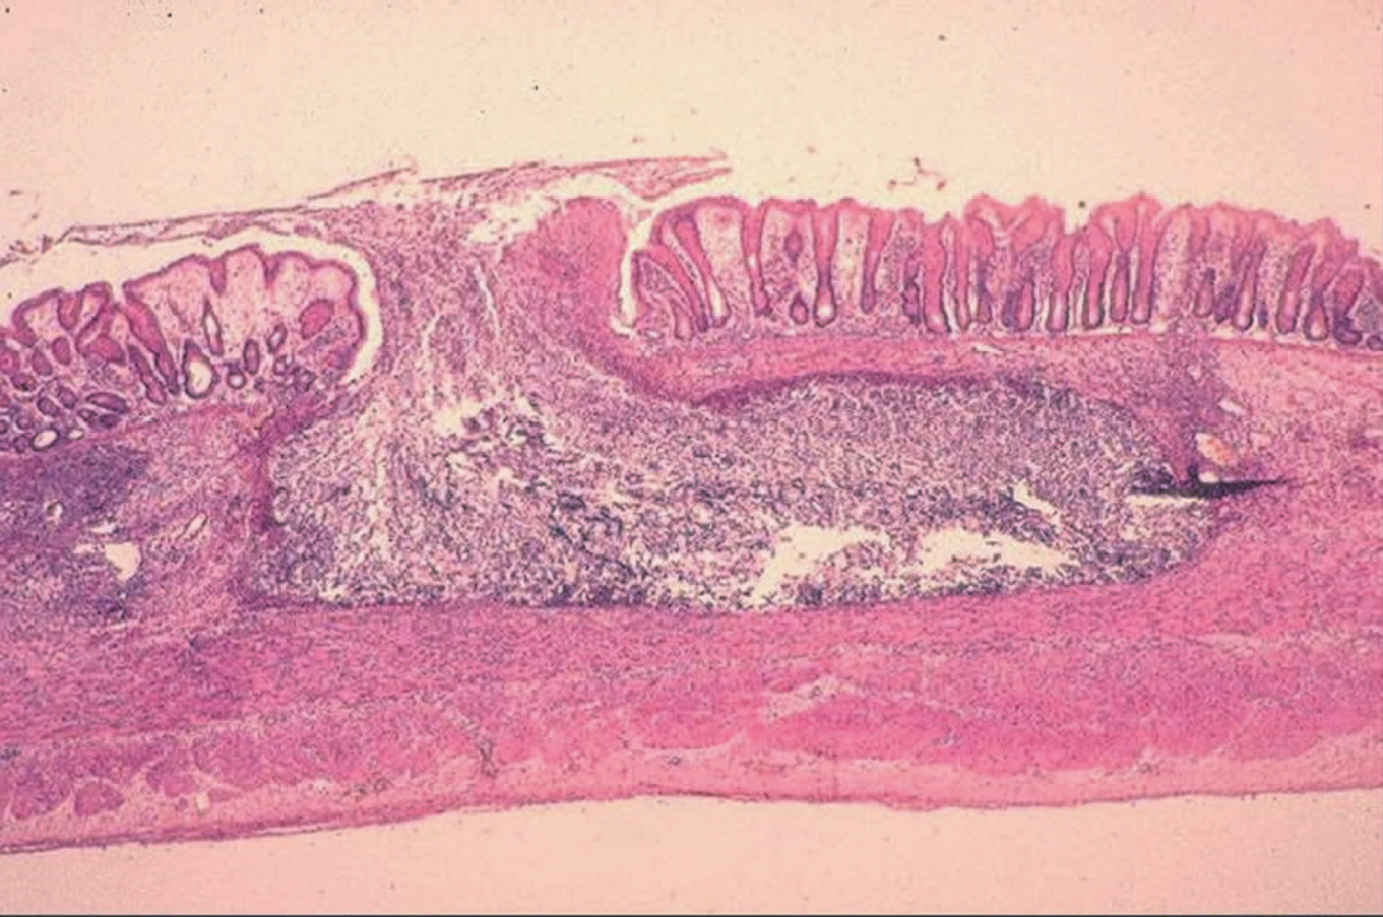
\includegraphics{./images/Image00244.jpg}
 \captionsetup{justification=centering}
 \caption{结肠阿米巴病(HE染色,低倍)\\ {\small 结肠壁见一口小底大的烧瓶状溃疡}}
\label{fig15-1}
  \end{figure}

镜下观:在溃疡底部和边缘可见无结构的液化性坏死组织,周围组织的炎症反应轻微,仅见充血、出血及少量淋巴细胞、浆细胞和巨噬细胞浸润。如有继发感染,溃疡的边缘可见有多量中性粒细胞浸润。在坏死组织与正常组织交界处,常可找到阿米巴滋养体。阿米巴滋养体一般呈圆形,体积通常较巨噬细胞大,有一个球形的泡状核,直径4~7
μm,胞浆略显嗜碱性,其中可见被吞噬的红细胞、淋巴细胞和组织碎片等(图\ref{fig15-2}),如无继发感染,则溃疡之间黏膜正常或仅有轻度渗出性炎。

临床上,急性期因结肠受炎症刺激,肠蠕动增强,黏液分泌增加,表现为腹痛、腹泻和大便次数增多。大便内含大量黏液、血液及坏死溶解的肠壁组织,呈紫红或暗红色的糊状,伴腥臭味。粪检时也找到阿米巴滋养体。本病的直肠及肛门病变较轻,故里急后重症状不如细菌性痢疾明显,全身中毒症状也很轻微,二者的区别见表\ref{tab15-1}。急性期多数可治愈,溃疡经肉芽组织填补、黏膜上皮再生覆盖而愈合,少数病例可出现肠出血和肠穿孔等并发症,也可因治疗不及时或不彻底而转入慢性期。

\begin{figure}[!htbp]
 \centering
 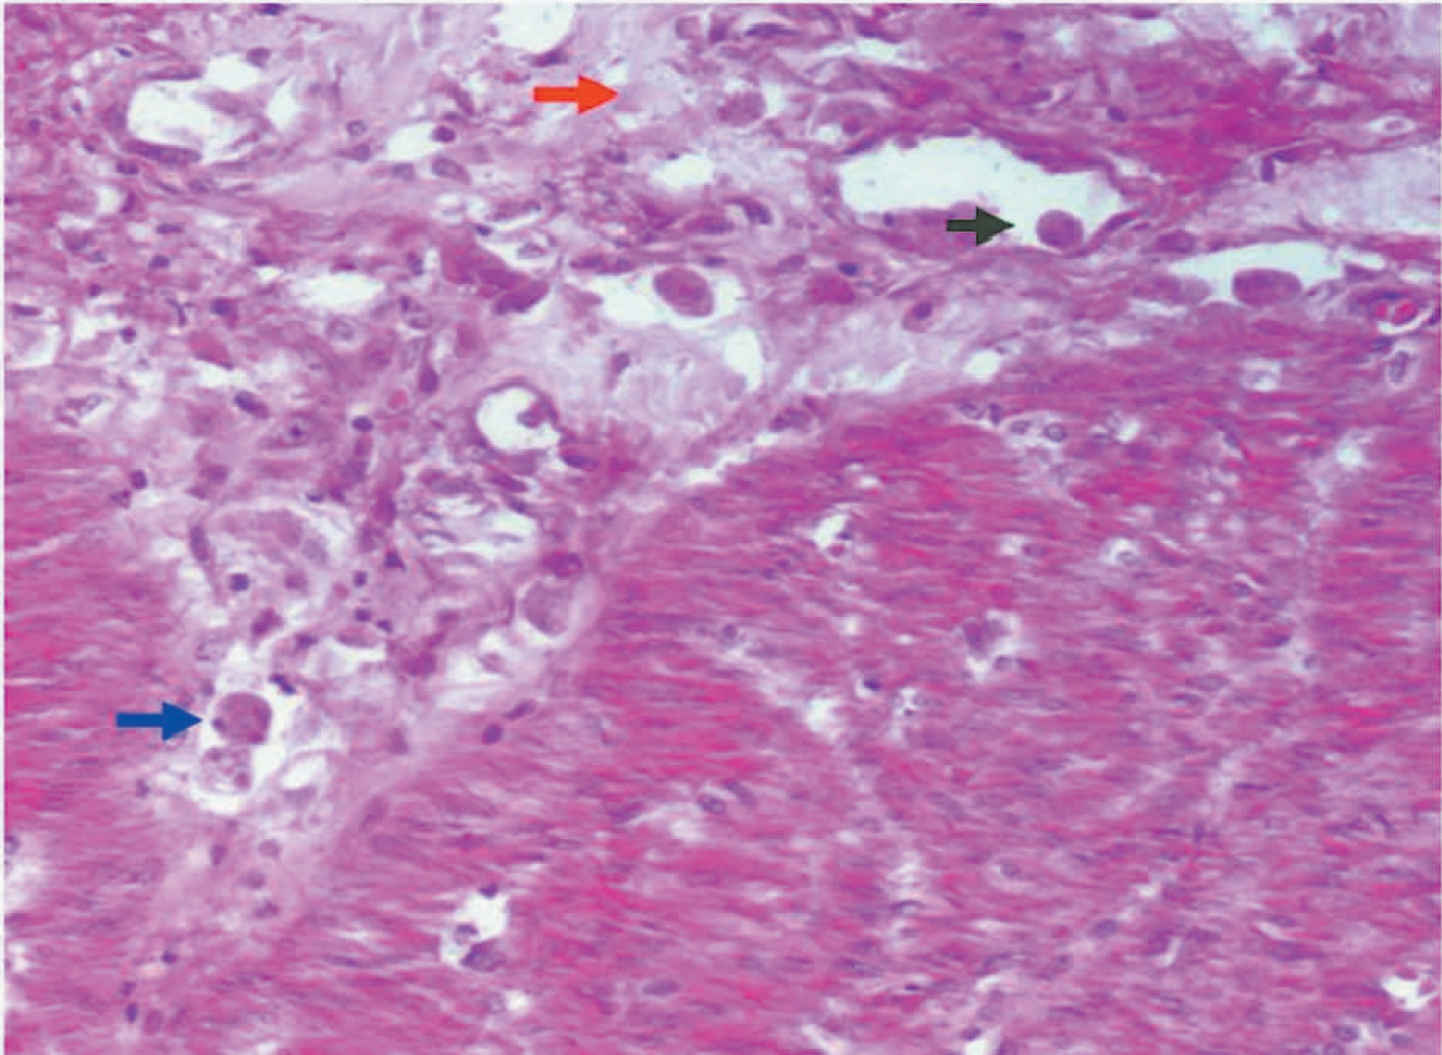
\includegraphics{./images/Image00245.jpg}
 \captionsetup{justification=centering}
 \caption{阿米巴病(HE染色,高倍)\\ {\small 红箭示肠溃疡底部的液化性坏死。黑箭示阿米巴滋养体侵入小血管内。蓝箭示阿米巴滋养体。}}
\label{fig15-2}
  \end{figure}

\begin{table}[ht]
	\caption{肠阿米巴病和细菌性痢疾的区别}
	\label{tab15-1}
	\centering
	\begin{tabular}{lp{5cm}p{5cm}}
	\toprule
	&肠阿米巴病&细菌性痢疾\\\\
	\midrule
	病原体&溶组织内阿米巴&痢疾杆菌\\
好发部位 & 盲肠、升结肠&乙状结肠、直肠\\
病变性质&局限性坏死性炎&弥漫性假膜性炎\\
溃疡形态&一般较深,烧瓶状&一般较浅,不规则\\
溃疡边缘&潜行性、挖掘状&不呈挖掘状\\
溃疡间黏膜&大致正常&炎性假膜覆盖\\
肠道症状 &右下腹压痛,腹泻不伴里急后重&左下腹压痛,腹泻常伴里急后重\\
全身症状&轻,很少发热 &重,常有发热\\
粪便检查&腥臭味,暗红色果酱样,镜检红细胞多,能找到阿米巴滋养体&粪质少,黏液脓血便,鲜红色,可见脱落的假膜,镜检脓细胞多\\
	\bottomrule
	\end{tabular}
\end{table}


\paragraph{慢性期病变}
肠壁病变较急性期复杂,有的溃疡已愈合或愈合后又重新发生坏死,出现新旧病灶共存,因此组织坏死、溃疡、肉芽组织增生和瘢痕形成反复交错发生,最后使肠黏膜完全失去正常结构。肠壁因纤维组织增生而增厚变硬,甚至引起肠腔狭窄,局部组织过度增生还可导致息肉形成,有的因肉芽组织增生过多而形成局限性包块,称为阿米巴肿(amoeboma),多见于盲肠,临床上易误诊为结肠癌。慢性期病人和包囊携带者是阿米巴病的主要传染源。

临床上,慢性期病人的症状较轻微,可能只有轻度腹泻、腹痛、腹部不适等肠功能紊乱症状,常反复发作,经久不愈。长期不愈合患者可引起全身营养不良和消瘦。

肠阿米巴病的并发症有肠穿孔、肠出血、肠腔狭窄、阑尾炎及阿米巴肛瘘等,也可引起肝、脑、肺等肠外器官的病变。少数病人可因肠道溃疡过深而引起穿孔,因本病病变发展缓慢,在穿孔前溃疡底的外膜层常与周围组织粘连,故穿孔时仅形成局限性脓肿,很少引起弥漫性腹膜炎。肠出血较常见,多因病变破坏肠壁小血管所致,但很少累及大血管。

\subsection{肠外阿米巴病}

肠外阿米巴病(extraintestinal
amoebiasis)以肝、肺、脑为最常见,也可累及脑膜、皮肤和泌尿生殖系统等。

\subsubsection{阿米巴肝脓肿}

在肠外阿米巴病中最常见,大多发生于肠阿米巴病发病后1~3个月内,少数可在肠道症状消失数年后发生。阿米巴滋养体一般通过侵入肠壁小静脉血行播散抵达肝脏。偶尔也可直接进入腹腔再入侵肝脏,引起肝脏病变。局部肝组织由于滋养体破坏和溶解而发生液化性坏死,形成所谓“脓肿”。阿米巴肝脓肿以单个多见,早期为多发性脓肿,以后互相融合形成单个大脓肿。病症多位于肝右叶,其原因可能与肝右叶体积大(约占肝总体积4/5),滋养体进入的机会多所致,以及原发病灶大多位于盲肠、升结肠,该处血流由于门静脉分流现象大多进入肝右叶有关。

肉眼观:脓肿大小不等,大者几乎占据整个肝右叶,可呈圆形或不规则形,脓肿壁不光滑,常附有未彻底液化坏死的肝组织,呈特征性破棉絮状(图\ref{fig15-3})。脓肿内容物为液化坏死的肝组织和陈旧性出血混合而成的“巧克力”样物质,而并非脓液。炎症反应不明显。

\begin{figure}[!htbp]
 \centering
 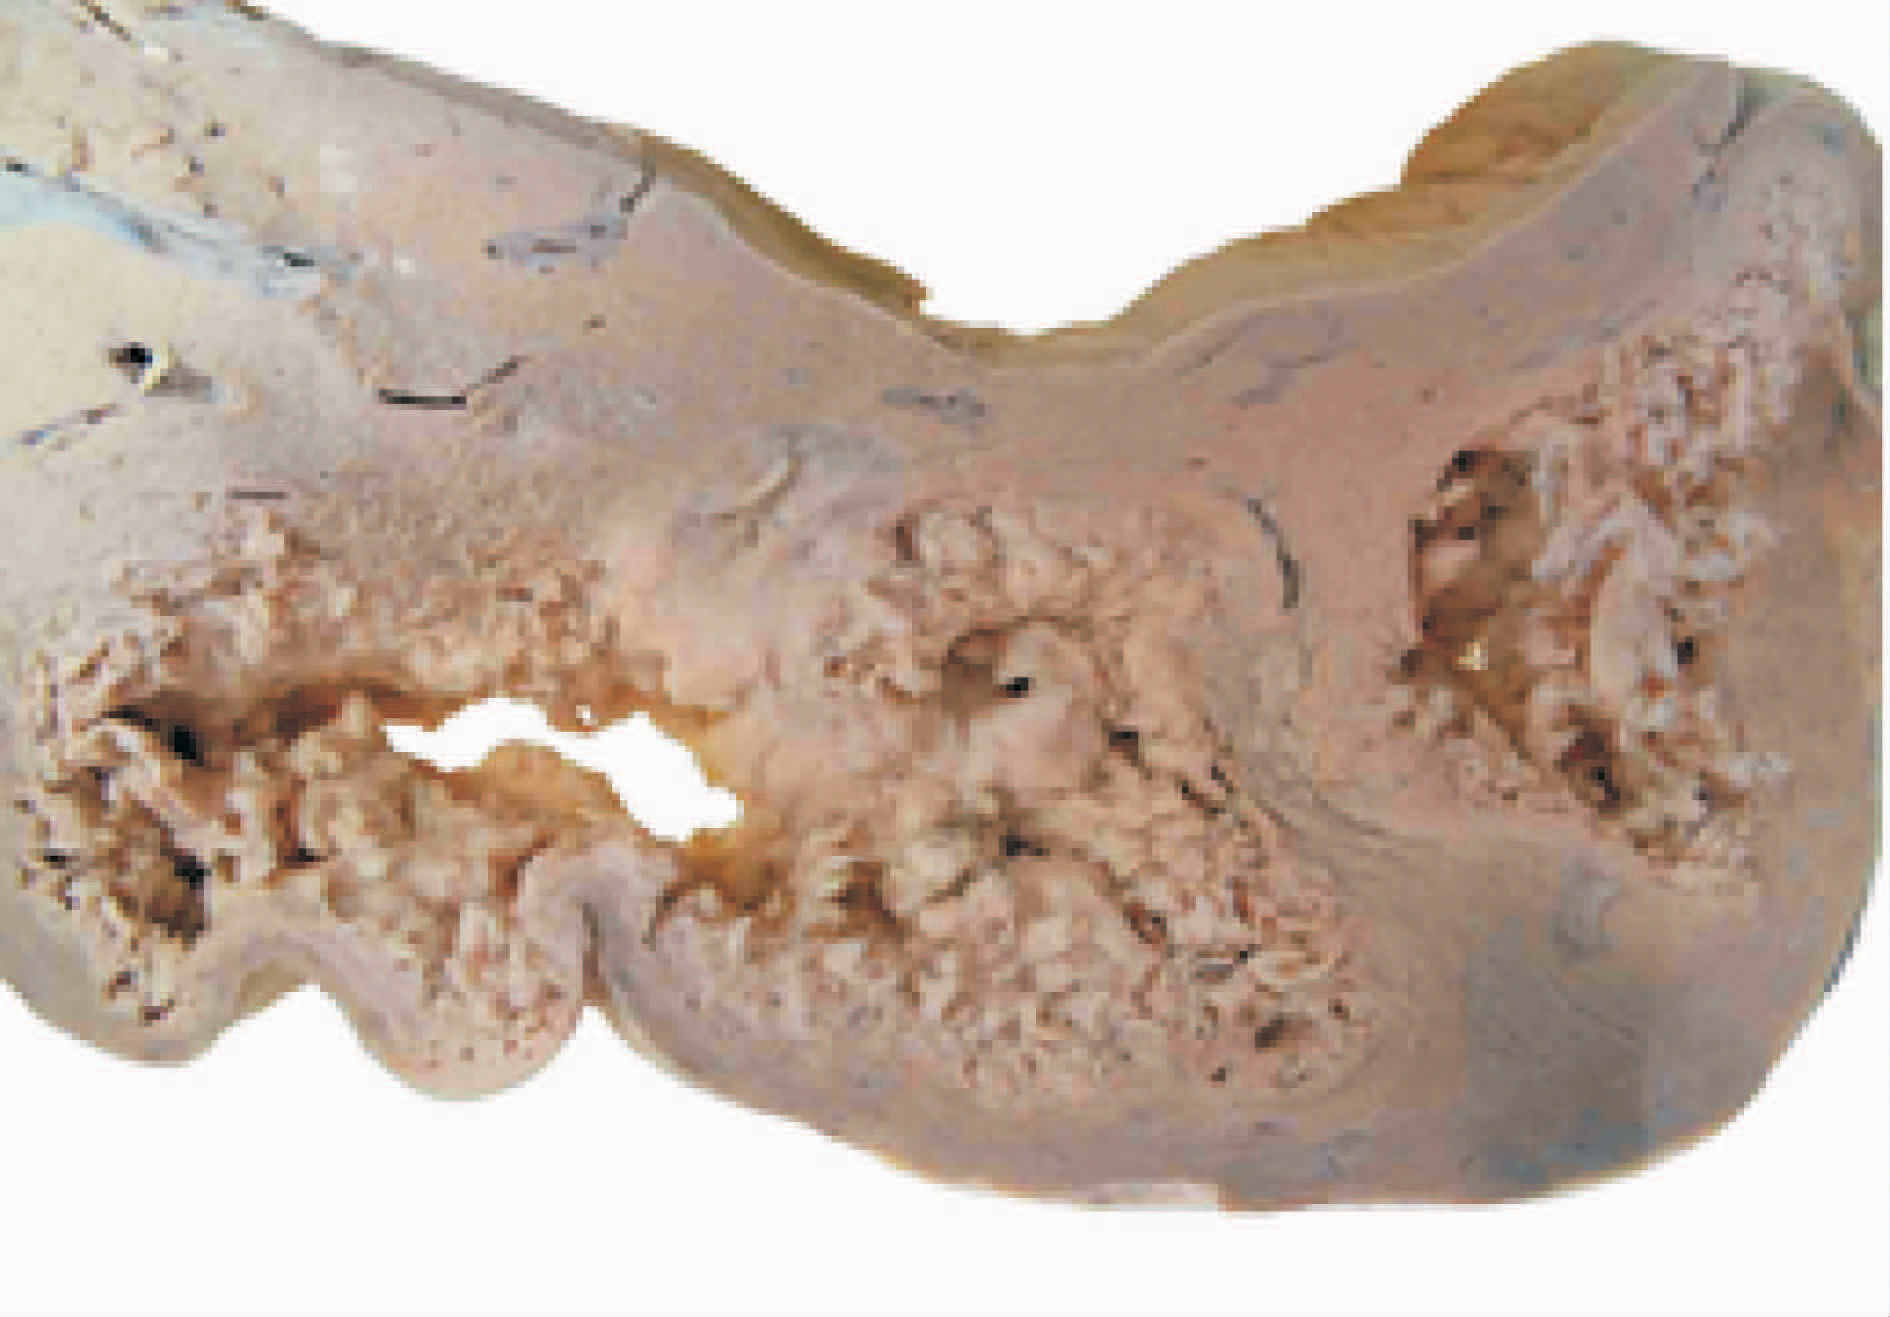
\includegraphics{./images/Image00247.jpg}
 \captionsetup{justification=centering}
 \caption{阿米巴性肝脓肿\\ {\small 脓肿壁不光整,呈破棉絮样}}
\label{fig15-3}
  \end{figure}

镜下观:脓腔内为液化坏死的“巧克力”样物质,脓肿壁为未彻底液化坏死的组织,仅有少量淋巴细胞、浆细胞和巨噬细胞浸润,大滋养体多在脓肿壁周围。若伴化脓菌继发感染,病变与真性脓肿相似,有时很难区分。慢性脓肿周围可有肉芽组织及纤维组织包绕。

临床上,阿米巴肝脓肿症状体征的轻重与脓肿的位置、大小以及是否伴有感染有关。常表现为长期不规则发热,伴有上腹痛及肝肿大和压痛,并有发热、黄疸、全身消耗等症状和体征。阿米巴肝脓肿若未能及时诊断和治疗,病灶继续扩大向四周组织破溃,可引起相应部位的病变,如肺脓肿、膈下脓肿、脓胸及腹膜炎等。

\subsubsection{阿米巴肺脓肿(amoebic lung abscess)}

发生率远低于阿米巴肝脓肿,临床上少见。绝大多数肺脓肿是由于肝脓肿穿过横膈直接蔓延而来(肝源性),故右肺下叶多见。少数为阿米巴滋养体由直肠壁经痔静脉、下腔静脉入肺,或经淋巴道、上腔静脉入肺(肠源性)。肺脓肿与肝脓肿的病灶形态特点相似。脓肿腔内坏死物质可破溃入支气管,坏死物被排出后形成空洞;溃破入胸腔可形成胸膜支气管痿等。临床上患者有类似肺结核的症状,如咳嗽、呼吸困难、咯血或咳出棕褐色脓样痰,其中可检见大量阿米巴滋养体。

\subsubsection{阿米巴脑脓肿(amoebic brain abscess)}

极少见,多因肠、肝和肺部的阿米巴滋养体经血流进入脑而引起,故本病多合并肠、肝或肺阿米巴病。脑脓肿常为多发性,多见于大脑半球。脓腔内充满咖啡色坏死液化物,周围常有慢性炎细胞浸润和增生的神经胶质细胞构成的脓肿壁。病人可有发热、头痛、昏迷等症状。此病预后极差。

脑膜、皮肤、肛门、阴道和子宫颈等器官也可被侵犯引起相应的病变。

\section{血吸虫病}

血吸虫病(schistosomiasis)是由血吸虫寄生于人体引起一种严重的地方性寄生虫病。寄生于人体的血吸虫主要有日本血吸虫、曼氏血吸虫和埃及血吸虫三种,在我国仅有日本血吸虫病流行,通常将日本血吸虫病简称为血吸虫病。本病主要流行于我国长江流域及其以南的十三个省市的广大水稻种植区。本病在我国流行历史久、范围广,对广大劳动人民的健康危害极大。新中国成立之后,积极开展了防治工作,情况虽已大为改善,但近年来有些地区的发病率有所回升或发现新的疫区,因此,血吸虫病的防治工作任重而道远。

\begin{framed}
{案例15-2}

{【病例摘要】}

李某,男,40岁,江苏徐州人。因发热、腹痛、脓血便2个月余入院。

现病史:打工湖北,多次下河游泳,足、手臂等处皮肤出现小米粒状的红色丘疹,发痒,未重视。几天后发烧,咳嗽,痰中偶带血丝,自服感冒药后症状逐渐消失。一个多月后再次发热,便中有脓血,每天4~6次,伴右上腹部轻微胀痛,食欲减退、体重减轻。曾多次到当地医院就诊,按痢疾处理,疗效欠佳,遂到上级医院就诊。

既往史:既往体健。

查体:体温39℃;消瘦病容,神志清楚;心、肺(-),腹部稍膨胀,肝剑突下3
cm,有压痛,脾可触及,四肢(-),体重65 kg。

化验:血常规白细胞计数2×10{8}
,中性粒细胞48%,淋巴细胞35%,单核细胞17%,尿常规正常。胸部摄片:正常。

{【问题】}

1. 根据上述病史、体检及化验结果,你认为其最可能患何病?

2. 患者还应当进行哪些检查以便确诊?

3. 患者体内可能有哪些病理变化?任其发展,可能出现哪些后果?
\end{framed}

血吸虫病其病变主要发生在结肠和肝脏,晚期血吸虫病患者常发展为肝硬化并出现较严重的门静脉高压。临床上常出现腹水、巨脾、食管静脉曲张等症状。

\subsection{病因及感染途径}

日本血吸虫为本病的病原体,其生活史可分为虫卵、毛蚴、尾蚴、童虫及成虫等阶段。成虫以人体或其他哺乳动物如猪、猫、狗、牛、羊、马等为终宿主,毛蚴至尾蚴的发育繁殖阶段以钉螺为中间宿主。血吸虫传播必须具备3个条件,即带虫卵的粪便入水,钉螺的孳生以及人体接触疫水。

病人或病畜排出的粪便中的血吸虫卵进入水中,在适当的条件下孵化出毛蚴,毛蚴钻入钉螺体内,发育成为尾蚴;尾蚴在水中游弋,当人畜与疫水接触时,尾蚴借其头腺分泌的溶组织酶作用和机械运动,很快钻入皮肤或黏膜,并脱去尾部转变为童虫;童虫经淋巴管或小静脉进入血液循环,先经右心而到达肺,以后经肺静脉进入大循环向全身散布,只有进入肠系膜静脉的童虫,才能继续发育成为成虫。童虫三周左右即可发育为成虫,雌、雄成虫在肠系膜静脉内交配产卵,部分虫卵顺血流流入肝,部分则逆血流至肠壁。虫卵在组织内沉积,约11天发育为成熟虫卵,形成急、慢性虫卵结节,而引起相应的病理变化。

\subsection{基本病变及发病机制}

在血吸虫感染过程中,尾蚴、童虫、成虫及虫卵等均可引起宿主受感染部位病变,但其中以虫卵引起的病变最严重、危害最大。造成损害的原因和机制主要是不同虫期血吸虫释放的抗原诱发宿主的免疫反应所致。

\paragraph{尾蚴引起的病变------尾蚴性皮炎}
尾蚴钻入皮肤后,引起皮肤出现炎症反应称尾蚴性皮炎(cercarial
dermatitis)。一般在尾蚴钻入皮肤后数小时至2~3天内发生,表现为入侵局部奇痒的红色小丘疹,经数天后可自然消退。镜下见真皮毛细管扩张充血、水肿及出血,起初有嗜酸性粒细胞和少量中性白细胞浸润,以后主要为单核细胞浸润。目前认为主要与Ⅰ及Ⅳ型变态反应有关。

\paragraph{童虫引起的病变}
童虫在体内移行时可引起血管炎和血管周围炎,尤以肺组织受损最为明显,部分童虫可穿破肺泡壁毛细血管,游出到肺组织中,引起肺组织局部点状出血及嗜酸性粒细胞浸润,但病变一般轻微而短暂。病人可出现发热、一过性咳嗽和痰中带血等症状。童虫引起各器官的病变除与童虫的机械作用有关外,还与其代谢产物或虫体死亡后蛋白分解产物所致组织的变态反应有关。童虫表面有特异性抗原,嗜酸性粒细胞和巨噬细胞通过抗体依赖性细胞介导的细胞毒性反应对童虫有杀伤作用。因此,当宿主再次感染尾蚴时有一定免疫力。

\paragraph{成虫引起的病变}
成虫对机体的损害作用较轻,原因可能是成虫的表面含有宿主的抗原,被宿主认为是“自我”组织而逃避了免疫攻击。主要表现为静脉内膜炎、静脉周围炎和虫体抗原成分或代谢产物引起的过敏反应。病人可出现轻度贫血、嗜酸性粒细胞增多和脾肿大。肝、脾单核巨噬细胞吞噬血吸虫成虫摄取红细胞后分解形成黑褐色血红蛋白色素(血吸虫色素)。死亡的成虫周围可形成嗜酸性脓肿。

\paragraph{虫卵引起的病变}
虫卵沉着所造成的损害是血吸虫病的主要病变。寄生于门脉系统的成虫的虫卵常沉积于结肠、肝脏,异位损害较多见于肺部及脑部。未成熟虫卵因其中毛蚴不成熟,无毒性分泌物,所引起的病变较轻;含毛蚴的成熟虫卵因毛蚴头腺分泌物中的抗原物质可引起以增生和坏死为特征的眼中变态反应,往往引起虫卵结节形成。按其病变发展过程可分为急性和慢性虫卵结节。

(1)急性虫卵结节:是由成熟虫卵的毛蚴释放出可溶性虫卵抗原引起的一种急性渗出、坏死性病灶。肉眼观:灰黄色、粟粒至黄豆大小的小结节。镜下观:结节中央为多少不等的成熟虫卵,虫卵的卵壳上有放射状嗜酸性棒状小体,也称为Hoeppli现象,免疫荧光法证实其为抗原抗体免疫复合物。虫卵周围是一片无结构的颗粒状坏死物质及大量嗜酸性粒细胞浸润,形态状似脓肿,故又称“嗜酸性脓肿”。在坏死组织间可见菱形或多面形有折光性的蛋白质晶体,即夏柯-莱登(charcot-Leyden)结晶(图\ref{fig15-4}),是由嗜酸性粒细胞的嗜酸颗粒互相融合而成。以后“脓肿”周围开始形成新生肉芽组织,随着虫卵内毛蚴死亡,病变逐渐演变为慢性虫卵结节。

\begin{figure}[!htbp]
 \centering
 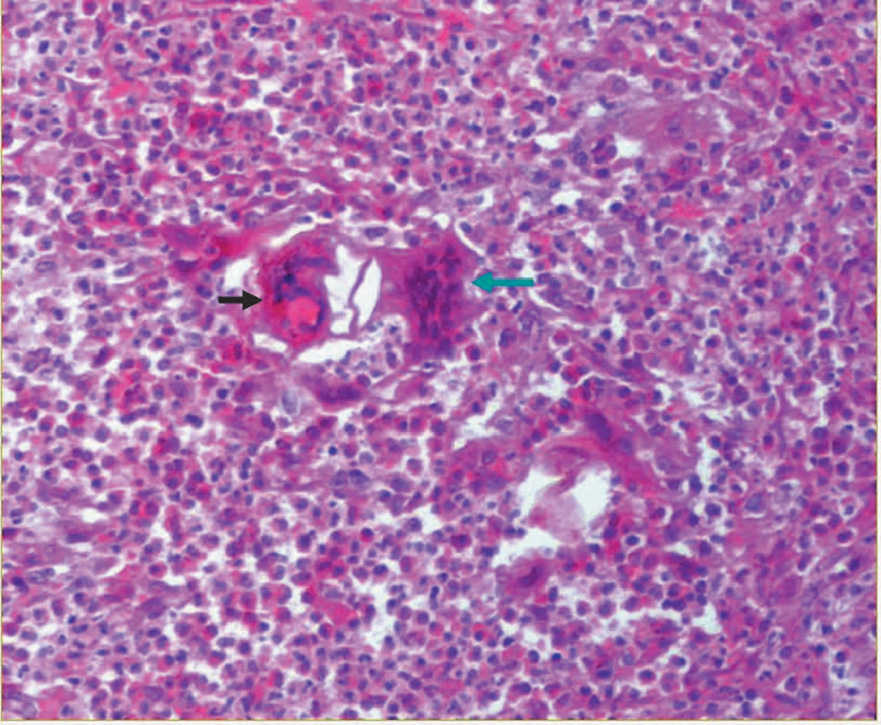
\includegraphics{./images/Image00248.jpg}
 \captionsetup{justification=centering}
 \caption{急性血吸虫虫卵结节(嗜酸性脓肿)(HE染色,高倍)\\ {\small 结节中央可见血吸虫虫卵(黑箭头)和多核巨细胞(蓝箭头),周围有大量的坏死组织及嗜酸性粒细胞聚集。}}
\label{fig15-4}
  \end{figure}

(2)慢性虫卵结节:急性虫卵结节经过10余天后,虫卵内毛蚴死亡,坏死物质被吸收,逐渐转变为慢性虫卵结节。镜下观:结节中央为死亡的虫卵,卵壳破裂或钙化,周围出现由组织细胞转变而来的类上皮细胞、多核异物巨细胞和淋巴细胞及少量嗜酸性粒细胞。其形态类似结核性肉芽肿,故又称为假结核结节(pseudotubercle),即慢性虫卵结节(图\ref{fig15-5})。最后,结节发生纤维化玻璃样变,中央的卵壳碎片及钙化虫卵可长期存留。肉芽肿的形成,一方面有利于隔离及中和虫卵释放的抗原和毒性物质,起到局部免疫屏障作用;另一方面,该肉芽肿的纤维化却能破坏宿主正常组织并导致器官纤维化。

\begin{figure}[!htbp]
 \centering
 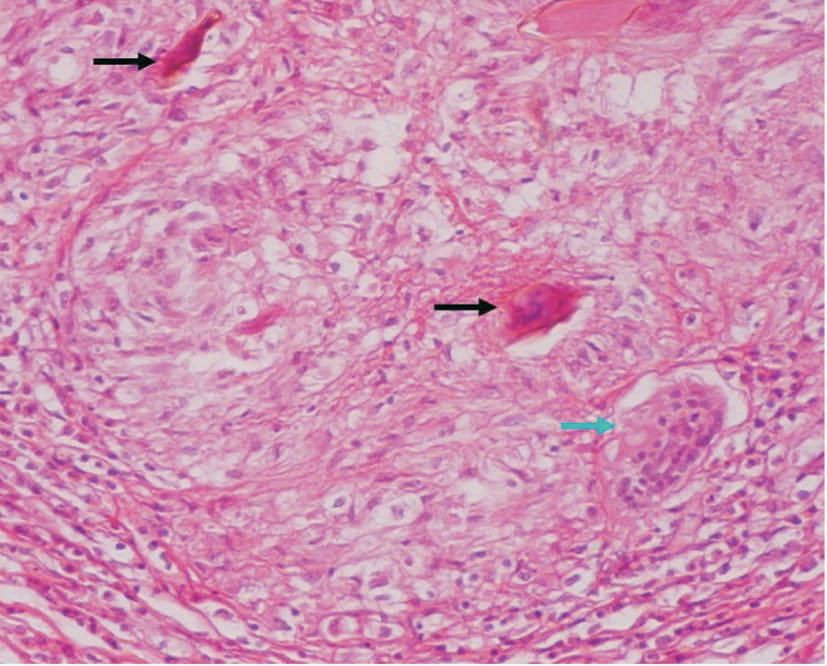
\includegraphics{./images/Image00249.jpg}
 \captionsetup{justification=centering}
 \caption{慢性血吸虫虫卵结节(假结核结节)(HE染色,高倍)\\ {\small 结节中央的血吸虫虫卵已死亡(黑箭头),周围大量类上皮细胞,最外方为淋巴细胞及成纤维细胞。虫卵右下方为一多核异物巨细胞(蓝箭头)}}
\label{fig15-5}
  \end{figure}


\subsection{主要器官的病变及临床病理联系}

\subsubsection{肠}

血吸虫成虫多寄生于肠系膜下静脉及痔上静脉,故病变可累及全部结肠,但以乙状结肠、降结肠和直肠最显著,小肠病变罕见。

\paragraph{急性期病变}
肉眼观:由于虫卵沉积于黏膜及黏膜下层引起急性虫卵结节。肉眼可见肠黏膜充血水肿及灰黄色细颗粒扁平隆起的病灶。随后,病灶中央组织坏死脱落,形成大小不一、边缘不规则浅表溃疡,虫卵可随坏死组织脱落而排入肠腔,并随着粪便排出成为污染源。镜下观:黏膜及黏膜下层有成堆虫卵堆积及急性虫卵结节形成,尤以黏膜下层最明显。临床上出现腹痛、腹泻等痢疾症状。粪便可查见虫卵或孵化出毛蚴,有助于诊断。

\paragraph{慢性期病变}
肉眼观:因虫卵反复沉积,肠壁反复发生溃疡和纤维化,导致肠壁不规则增厚、变硬甚至肠腔狭窄,引起肠梗阻。肠黏膜上皮增生还可形成多发性小息肉,肠黏膜粗糙不平、萎缩、皱襞消失(图\ref{fig15-6})。由于肠壁结缔组织增生,使以后到达肠壁的虫卵难以排入肠腔,故晚期患者粪便中不易查到虫卵,可查见处于不同阶段的急、慢性虫卵结节。肠道慢性血吸虫病可并发结肠癌,发生部位也多在乙状结肠及直肠,可由息肉演变而来。

\begin{figure}[!htbp]
 \centering
 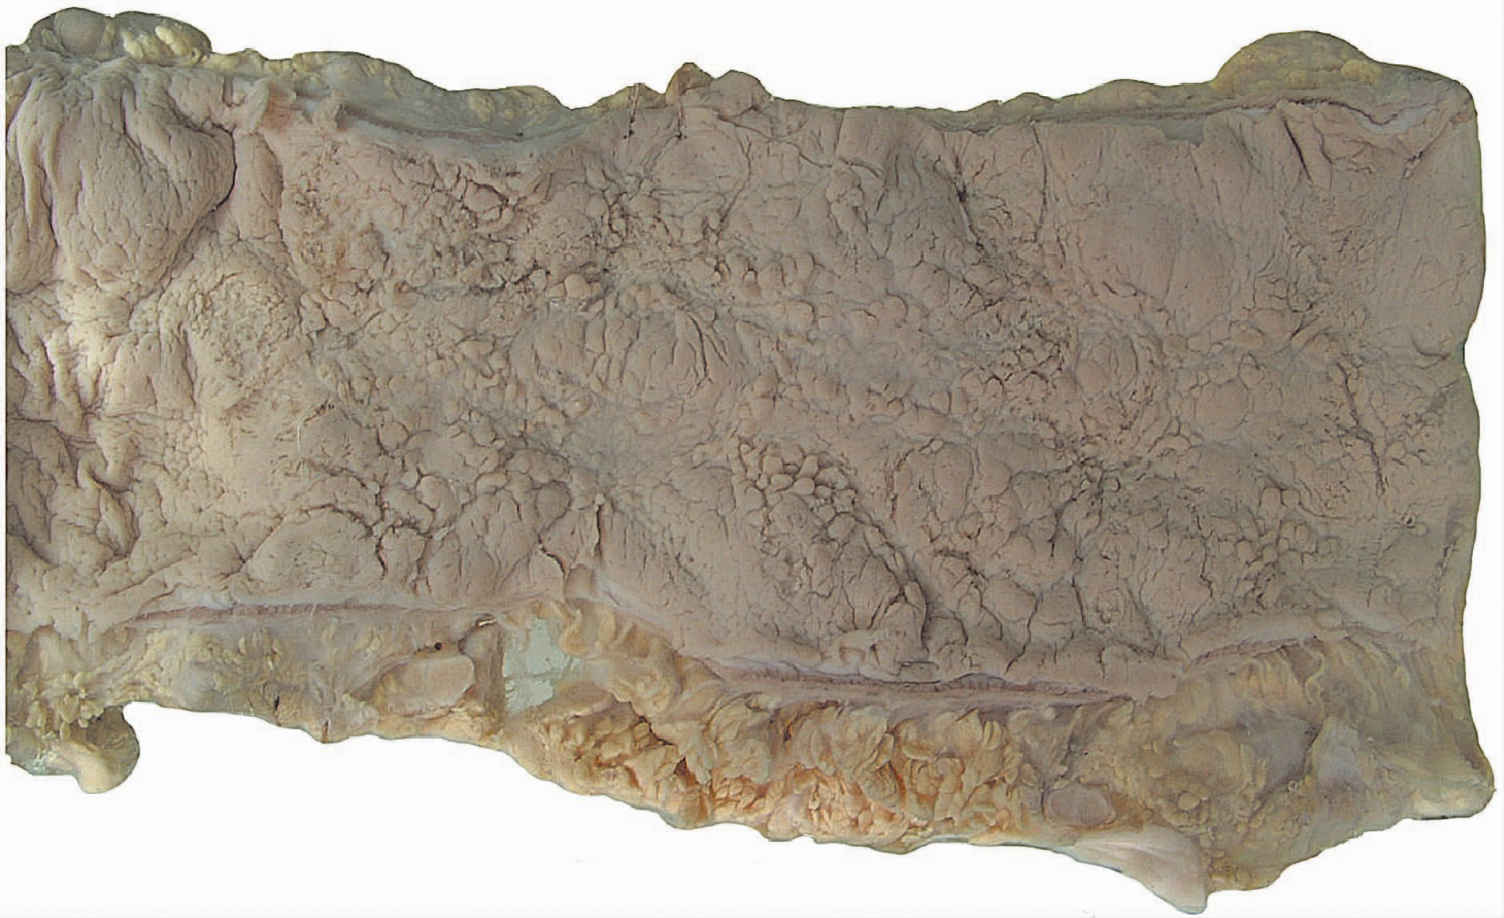
\includegraphics{./images/Image00250.jpg}
 \captionsetup{justification=centering}
 \caption{血吸虫病的结肠病变\\ {\small 肠黏膜粗糙不平、萎缩、皱襞消失,形成多发性小息肉}}
\label{fig15-6}
  \end{figure}

\subsubsection{肝脏}

虫卵随门静脉血液进入肝脏,沉积在汇管区的门静脉小分支引起病变。以肝左叶病变更明显。

\paragraph{急性期病变}
肉眼观:肝脏轻度肿大,表面光滑,肝表面或切面有多个灰黄色或灰白色粟粒或绿豆大小结节。镜下观:汇管区附近见较多急性虫卵结节,肝小叶边缘肝窦充血,肝细胞水肿,枯否细胞内可见黑褐色血吸虫色素沉着。

\paragraph{慢性期病变}
由于肝内虫卵结节形成及纤维化病变反复交替出现,最终导致肝内大量纤维组织增生,肝质地变硬,而形成所谓血吸虫性肝硬化。肉眼观:肝体积缩小,质地变硬,表面有许多大小不一的结节及散在浅沟纹。切面汇管区增宽,增生的结缔组织沿门静脉分支呈树枝状分布,故有干线型或管道型肝硬化之称。由于病变主要发生在汇管区,肝小叶未遭受严重破坏,故不形成假小叶。镜下观:汇管区有较多的慢性虫卵结节,伴有纤维组织增生和慢性炎细胞浸润(图\ref{fig15-7}),肝小叶结构大多完好,肝细胞有不同程度萎缩,但无明显的坏死、再生及再生结节形成,小胆管增生也不明显。临床上由于门静脉分支虫卵阻塞、静脉内膜炎、血栓形成及静脉周围纤维组织增生,使门静脉分支阻塞和受压,最终导致门静脉高压。因肝内门静脉的阻塞是窦前性的,故门静脉高压较肝炎后肝硬化时更为明显。临床上常出现腹水、巨脾、食管静脉曲张等。

\begin{figure}[!htbp]
 \centering
 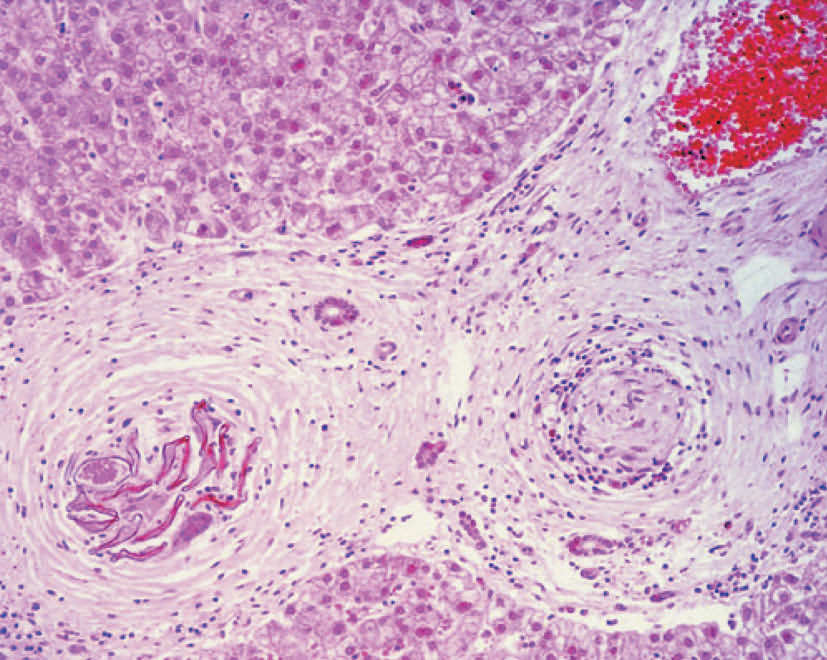
\includegraphics{./images/Image00251.jpg}
 \captionsetup{justification=centering}
 \caption{血吸虫病肝硬化(HE染色,低倍)\\ {\small 汇管区可见两个已发生纤维化之假结核结节}}
\label{fig15-7}
  \end{figure}

\subsubsection{脾脏}

在感染早期,因成虫的代谢产物刺激,单核巨噬细胞增生,引起轻度脾肿大;晚期由于门静脉高压导致慢性脾淤血和结缔组织增生,脾脏体积中到重度增大,甚至形成巨脾。脾脏重量可达1
000 g,甚至4 000
g。肉眼观:脾包膜增厚、质地坚韧,可发生脾周围炎。切面呈暗红色,质地坚韧,脾小梁增粗,脾小体多萎缩或消失,可见散在的黄褐色含铁结节,有时还可见多数陈旧性梗死灶。临床上病人往往出现贫血,白细胞和血小板减少等脾功能亢进症状。

\subsubsection{异位损害}

异位损害指虫卵或成虫游走或寄生在门静脉系以外的器官所致病变,引起异位损害,以肺、脑、皮肤较为多见。

\paragraph{肺}
除早期由童虫移行所致病变外,也可由虫卵沉积引起。部分急性病例肺内可出现多数急性虫卵结节,其周围肺泡出现炎症渗出物。X线检查似粟粒性肺结核。通常肺的变化轻微,虫卵大多通过门静脉与腔静脉或肝静脉之间的交通支带至肺部。

\paragraph{脑}
脑血吸虫病主要见于大脑顶叶,也可累及额叶和枕叶,其次为小脑。表现为虫卵结节形成和胶质细胞增生,结节周围脑组织常发生灶性软化、出血和血肿。急性期临床常表现为脑炎或脑血管意外症状;慢性期常表现为癫病发作。虫卵入脑途径,可能是虫卵经肺进入体循环,以栓子的方式到达脑部,也可能通过门静脉和椎静脉的交通支到达脑部。

\paragraph{血吸虫侏儒症}
儿童时期如果反复、大量感染血吸虫,可导致侏儒症。患者表现身材矮小,面容苍老,第二性征缺如,无生殖能力,但智力一般不受影响。原因可能为长期营养不良,严重肝损害,以致体内某些激素不能灭活,继发脑垂体功能低下,垂体前叶萎缩、坏死,并继发甲状腺、性腺、肾上腺萎缩,导致骨骼发育迟缓所致。

\section*{复习与思考}

{一、名词解释}

阿米巴肿 嗜酸性脓肿 假结核结节

{二、问答题}

1. 简述肠阿米巴病的病理变化及临床病理联系。

2. 列表区别细菌性痢疾与阿米巴痢疾。

3. 哪些疾病可引起肠道溃疡?各自溃疡的主要病变特点有哪些?

4. 简述血吸虫病的病理变化及主要脏器的病变特征。解释临床病理联系。